\documentclass[10pt,a4paper]{report}

\usepackage[utf8]{inputenc}
\usepackage{amsmath}
\usepackage{amsfonts}
\usepackage{amssymb}
\usepackage{graphicx}
\usepackage{color}
\usepackage{enumitem}
\usepackage[top=1cm, bottom=2cm, left=2cm, right=2cm]{geometry}

\usepackage{fancyhdr}
\pagestyle{fancy}

\fancyhead{}
\fancyfoot{} 
\lhead{ \hspace{0.1cm} M1 WI 2014-2015  \hspace{0.4cm} \vline}
\chead{METEOR}
\rhead{K.B - K.L - N.R}
\rfoot{\thepage}

\author{Kevin BASCOL, Kevin LAOUSSING, Nicolas REYNAUD}
\title{METEOR : \\ \vspace*{0.5cm} Le jeu de Dames}

\makeatletter
\renewcommand{\thesection}{\@arabic\c@section}
\makeatother

\begin{document}

\makeatletter
	\begin{titlepage}
	
	\centering
		{
		\vspace*{5cm}
		\hrule height 2pt
		\vspace{0.7cm}
		\Huge \textbf{\@title}}\\
		\vspace{0.7cm}
		\hrule height 2pt
		
		\vfill
		\vspace{1cm}
		\@author\\
		\end{titlepage}
\makeatother
\setcounter{secnumdepth}{4}
\setcounter{tocdepth}{3}
\renewcommand{\contentsname}{Sommaire}
\begingroup\makeatletter
\def\@makeschapterhead#1{%
  {\parindent \z@ \raggedright
    \normalfont
    \interlinepenalty\@M
    \Huge \bfseries  #1\par\nobreak
    \vskip 20pt% <---- à réduire pour avoir plus de place
  }}\makeatother
\tableofcontents
\endgroup
\thispagestyle{empty}
\setcounter{page}{0}
\newpage

\newgeometry{top=2cm, bottom=2cm, left=2cm, right=2cm}

\section{Introduction}
	Notre projet de METEOR consistait à implémenter un jeu à 2 joueurs. Nous avons choisi d'implémenter le jeu de Dames, un jeu suffisamment complexe et qui nous laisse apprécier l'efficacité de nos algorithmes.
Nous avons implémenté dans un premier temps l'affichage, les mouvements et les actions du jeu. Puis dans un second temps les règles et spécificités du jeu. Enfin une intelligence artificielle qui se base sur l'algorithme du MinMax, et de 3 fonctions heuristiques.
\section{Le jeu de Dame}
	\subsection{Description}
	Les dames ou jeu de dames est un jeu de société combinatoire abstrait pour deux joueurs où le but est de capturer ou d'immobiliser les pions de l'adversaire.
	\subsection{Configuration du jeu}
	Il existe plusieurs configuration du jeu de dames, pour notre projet nous avons choisi celle-ci :
	\begin{itemize}[label = $\blacktriangleright$]
		\item Damier :  10 x 10.
		\item Nombre de pions par camps : 20.
	\end{itemize}
	
	\subsection{Spécificités et règles de jeu implémentées}
		\subsubsection{Spécificités}
		
		\begin{itemize}[label = $\blacktriangleright$]
		\item Vérification des déplacements d'un pions/dame.
		\item Vérification des entrées utilisateurs.
		\item Déplacement de pions.
		\item Déplacement de reines.
		\item Saut de pion(s).
		\item Transformation de pions en reines.
		\end{itemize}
		
		\subsubsection{Règles de jeu implémentées}
		
		\begin{itemize}[label = $\blacktriangleright$]
		\item Les prises se font en avant et en arrière.
		\item La dame prend, à une distance quelconque, toute pièce suivie d'une ou plusieurs cases vides.
		\item Le déplacement des pions et reines se fait exclusivement en diagonale.
		\item Le déplacement des pions s'effectue uniquement dans un sens.
		\item Le déplacement des dames peut se faire dans les 2 sens. 
		\end{itemize}
\section{Algorithme du MinMax}
	Pour implémenter notre IA nous avons utilisé la méthode MinMax, universellement sollicitée dans les programmes comme les jeu d'échec, d'othello...

Le MinMax schématise le processus décisionnel que devrait suivre tout joueur : supposer que chaque joueur va, à chaque moment, prendre la décision qui est la meilleure pour lui. 
Ainsi, le processus utilisé par le programme correspond à l'alternance des décisions (IA/adversaire), et alterne les niveaux dits "maximisants", où le choix du coup à jouer appartient à l'IA, et les niveaux dits "minimisants", où le choix du coup appartient à son adversaire. La solution remontant au sommet est, avec certitude, le meilleur choix initial, compte tenu des meilleures réponses possibles de l'adversaire dans chaque cas.

Seules les évaluations de fin de branche sont nécessaires, les résultats remontant ensuite au sommet par alternance de maximisations et de minimisations.

\section{Heuristiques}

	\subsection{Avantage du nombre de pions (La meilleurs défense est l'attaque) }
	
	Cette heuristique part du principe que plus le joueur a un grand nombre de pion. Plus ses chances de gagner sont élevées. Ainsi son but est de manger le plus de pions possible parmi ceux de son adversaire.
	Cette stratégie est donc purement agressive. Qui plus est, si aucun coup pour manger n'est possible alors l'I.A. essayera de "creuser" un trou dans la défense ennemie en cherchant toujours à avancer vers la possibilité de faire une dame. \\
	
	Ceci implique également que l'I.A. essayera tout de même de diminuer le nombre de pion perdu.
	Car comme dit ci-dessus, moins nous avons de pions, plus nous nous approchons d'une défaite. \\
	
	Si 2 actions se présentent : 
	\begin{itemize}
		\item 1 - Nous pouvons prendre 3 pions.
		\item 2 - Nous pouvons prendre 2 pions.
	\end{itemize}
	l'I.A. prendra l'option numéro 1, même si son pion disparaît après.
	Ainsi cette stratégie essaie de rapprocher l'adversaire de la défaite en mangeant un maximum de ses pions ou à défaut en essayant d'attaquer l'ennemi.
	\subsection{Avantage des positions stratégiques}
		Dans cette heuristique nous avons choisi de donner des valeurs aux cases en fonction de leurs emplacement sur le damier. Les valeurs sont distribuées de la façon suivante:
		\begin{center}
			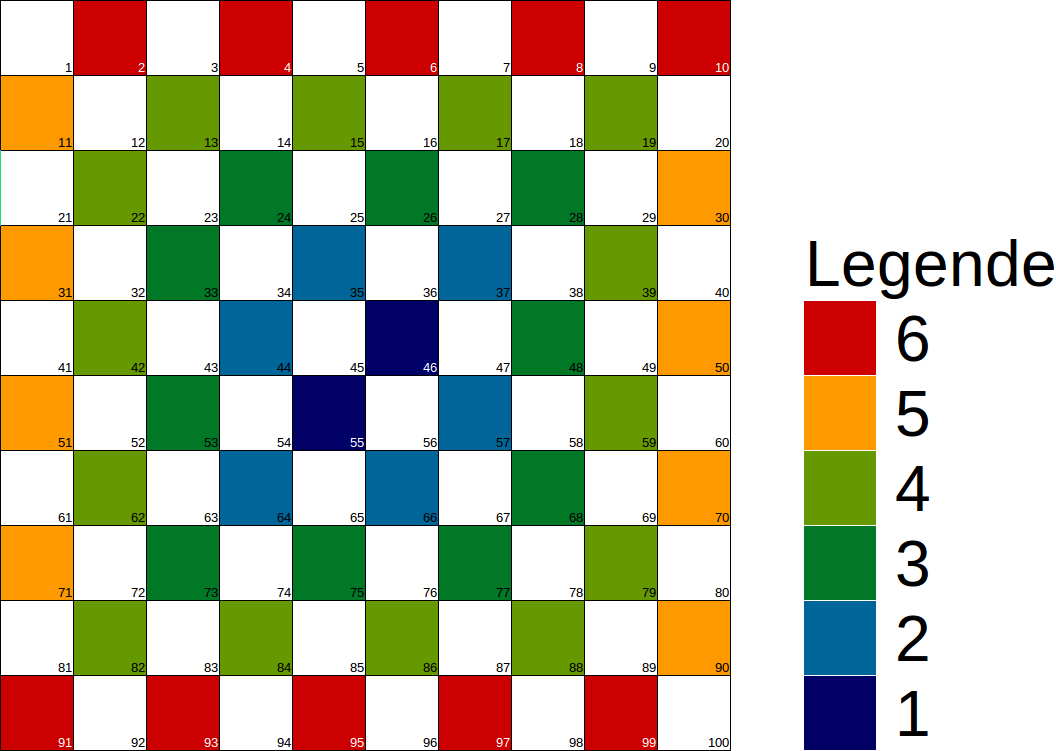
\includegraphics[scale=0.2]{valeursDamier.png}
		\end{center}
		Les cases les plus intéressantes sont celles du haut, pour créer des dames, et celles du bas, pour empêcher l'adversaire de le faire. Ensuite viennent les bordures permettant aux pions d'être hors d'atteinte de l'adversaire. Après on décrémente en se rapprochant du centre du plateau où il est plus facile de se faire prendre un pion.
		L'évaluation d'un instant du jeu se fait alors en ajoutant les valeurs des cases des pions de l'ordinateur, auxquelles on soustrait 10 pour chaque pion adverse pour respecter la règle de la prise obligatoire.
	\subsection{Avantage sur la fragilité défensive adverse }
	Cette heuristique se base sur le nombre de prises possibles : cela suppose que plus il y a de prises possibles (voir de rafles) dans le camp adverse, plus celui-ci est en difficulté car celui-ci ne peut défendre qu'une prise au prochain tour.\\
	L'évaluation d'un instant du jeu se fait alors en dénombrant le nombre de prises possibles de l'IA et le nombre de prises possibles de l'adversaire, et soustrayant les deux valeurs suivant celui qui a le "trait" ( c'est-à-dire celui qui doit jouer le tour).
	Pour cela, l'IA tente de reconnaître un "pattern" d'une prise pour chacun de ses pions. Par exemple un pattern de prise (diagonale bas gauche) peut être le suivant :\\
	\\
	$\mid n \mid b \mid x \mid b \mid\\
	------\\
	\mid b \mid o \mid b \mid n \mid\\
	------\\
	\mid n \mid b \mid n \mid b \mid\\
	------\\ $
	\\
	b : case blanche.\\
	n : case noire.\\
	x : le pion que joue l'IA.\\
	o : le pion qui va être pris.\\
\section{Remarques et difficultés}

L'une des difficultés principales du jeu de dames est son nombre de coups possibles partant d'un plateau de jeu. Ainsi avec une profondeur de 3 ou 4 il est courant de surcharger la pile d'exécution. \\

Autre remarque, le jeu implique énormément de règles et vérifications qui ont pris énormément de temps.
( déplacement d'un pion, ou saut d'un pion; déplacement d'une dame ou saut avec une dame). \\

\end{document}
